% Journal draft — generic template (plain article class). To move to a journal class (elsarticle, svjour3, acmart,
% IEEEtran, ...), keep the body and replace the preamble and the front matter.
% Build:  latexmk -pdf main.tex        Figures:  cd figures && python make_figures.py
% Notes for the authors are in \todo{...} (red); results to fill are "--".
\documentclass[11pt,a4paper]{article}
\usepackage[margin=2.5cm]{geometry}
\usepackage[T1]{fontenc}
\usepackage[utf8]{inputenc}
\usepackage{lmodern}
\usepackage{amsmath,amssymb}
\usepackage{graphicx}
\usepackage{booktabs}
\usepackage{xcolor}
\usepackage{tikz}
\usetikzlibrary{arrows.meta,positioning,shapes.misc}
\usepackage[numbers,sort&compress]{natbib}
\usepackage[colorlinks=true,linkcolor=blue!50!black,citecolor=blue!50!black,urlcolor=blue!50!black]{hyperref}

\newcommand{\todo}[1]{\textcolor{red}{[\textbf{TODO:} #1]}}
\newcommand{\fillme}{--}
\newcommand{\placeholder}[2]{\fbox{\parbox[c][#2][c]{#1}{\centering\small\color{gray} figure generated when the results are in}}}

\title{Reading the Source: Predicting the Reliability of Unseen News Outlets from the Text of Their Articles
\todo{working title}}
\author{John Bianchi \and \todo{co-authors and affiliations}}
\date{}

\begin{document}
\maketitle

\begin{abstract}
Source-level reliability ratings, such as the scores assigned by professional raters to news websites, are a key
signal against misinformation, but they cover only the outlets that the raters had time to review. We ask whether the
reliability of an outlet that a model has never seen can be estimated from the text of its articles alone. We build a
dataset of 25,524 articles from 226 political news outlets rated by NewsGuard, in which no two outlets share an owner,
and we remove from the text every explicit trace of the publisher: links, e-mail addresses, the outlet's own name and,
with a zero-shot named-entity recognizer, every news outlet and journalist. We predict the NewsGuard score (0--100) of
each outlet with a TF-IDF model, with two large language models used as frozen encoders (Qwen3-Embedding-8B and
Mistral-Small-24B) and with a fine-tuned ModernBERT, under an outlet-disjoint cross-validation stratified by score.
The best model, a ridge regression on the hidden states of Mistral-Small-24B, ranks the outlets with a Spearman
correlation of 0.735 and predicts their score with a mean absolute error of 15.8 points (no-text baseline: 22.6),
significantly better than TF-IDF (0.674 and 17.8 points); its advantage holds with any number of articles, and five
articles per outlet are enough to rank outlets better than TF-IDF reading all of them. The fine-tuned encoder does not
outperform TF-IDF, and masking every outlet and journalist leaves the results of the language models unchanged.
We release the code, the trained models and \emph{Publisher Evaluation}, a local tool that scores any article with
these models after the same anonymization and never lets a model score an outlet it was trained on.
\todo{polish.}
\end{abstract}

\noindent\textbf{Keywords:} news reliability; source credibility; misinformation; language models; text regression;
NewsGuard \todo{adapt to the journal}

% =====================================================================================================================
\section{Introduction}\label{sec:intro}

\todo{Motivation: misinformation is often judged at the level of the source; professional ratings (NewsGuard, Media
Bias/Fact Check) are reliable but slow and incomplete: new outlets, small outlets, outlets in other markets. A method
that estimates the rating of an outlet from what it publishes would extend these ratings and help prioritize the work
of the raters.}

\todo{The problem with previous text-based approaches: models can recognize the outlet instead of judging the text
(names, signatures, boilerplate, shared templates across sites of the same owner), and outlets seen in training can
leak into the test set; results are often reported per article and as classes. Cite \citep{zhou2021hidden} on hidden
biases in unreliable-news datasets and \citep{baly2018predicting,baly2020written} on media profiling.}

We study the problem in the setting that matters in practice: the outlet is \emph{unseen}, its articles are
\emph{anonymized}, and the target is the outlet's \emph{score} rather than a class. Our contributions are:
\begin{enumerate}
  \item a dataset of 226 political news outlets and 25,524 articles with NewsGuard 2026 scores, built with simple,
        reproducible rules: text extraction from the raw HTML, deduplication across outlets and one outlet per
        ownership group, so that sister sites never fall in different folds (Section~\ref{sec:data});
  \item an anonymization of the text based on a standard zero-shot named-entity recognizer, which masks every news
        outlet and journalist, not only the publisher (Section~\ref{sec:anon});
  \item a comparison of a TF-IDF model, two large language models used as frozen encoders and a fine-tuned encoder,
        evaluated per outlet with rank correlations and errors on the 0--100 scale, with paired bootstrap tests and
        as a function of the number of articles read per outlet (Sections~\ref{sec:method}--\ref{sec:results});
  \item the release of the code, of the trained models and of the out-of-fold predictions, and a local tool that
        applies the method to any article, with the same anonymization and a guard against training-data leakage
        (Section~\ref{sec:tool});
  \item \todo{the main finding, e.g. frozen large language models predict the score of unseen outlets better than
        TF-IDF, with few articles, and the result holds with a stricter anonymization.}
\end{enumerate}

% =====================================================================================================================
\section{Related work}\label{sec:related}

\paragraph{Source-level reliability and media profiling.}
\todo{Baly et al.\ \citep{baly2018predicting,baly2020written} (factuality and bias of media sources from articles,
Wikipedia, social media); NELA-GT \citep{gruppi2021nela} (source-level labels for articles); others to add.}

\paragraph{Shortcuts and leakage in news credibility datasets.}
\todo{Zhou et al.\ \citep{zhou2021hidden}: models learn the source, random article splits overestimate performance;
our outlet-disjoint, owner-disjoint split and anonymization address this. Other work on site-level vs article-level
evaluation.}

\paragraph{Language models as text encoders.}
\todo{Embedding models (Qwen3-Embedding \citep{zhang2025qwen3}), hidden states of decoder language models as features,
fine-tuned encoders (ModernBERT \citep{warner2024modernbert}); TF-IDF as a strong baseline for style and topic.}

\paragraph{Anonymization and named-entity recognition.}
\todo{Standard tools target personal data (e.g.\ Microsoft Presidio); our goal is different (mask the publisher, not
private individuals). GLiNER \citep{zaratiana2024gliner} as a zero-shot recognizer with free labels.}

% =====================================================================================================================
\section{Data}\label{sec:data}

\subsection{Labels}
NewsGuard \citep{newsguard} rates news websites with a score from 0 to 100, the weighted sum of nine journalistic
criteria (e.g.\ whether the site repeatedly publishes false content, corrects errors, discloses ownership), and with
five derived levels. We use the ratings of 2026 and keep the outlets whose only NewsGuard topic is
\emph{political news or commentary}. \todo{describe the criteria briefly; licence: the labels are not
redistributable.}

\subsection{Collection and cleaning}
In October 2026 we collected up to 200 recent articles per outlet from the websites of the NewsGuard-rated outlets,
saving the raw HTML of every page (5,113 outlets tried). From the 674 political outlets with at least one article we
built the dataset with the steps of Table~\ref{tab:cleaning}: the text is re-extracted from the HTML with trafilatura
\citep{barbaresi2021trafilatura} in precision mode (main text only); articles must be in English, have 100--1,500 words
and be published from 2025; exact and near duplicates (Jaccard similarity of word 5-grams $\geq 0.5$) are removed
across all outlets, keeping the oldest copy; an outlet needs at least 10 articles; finally, outlets that share the
NewsGuard owner or parent domain form an ownership group, and only the outlet with most articles is kept for each
group, so that networks of sister sites cannot appear on both sides of a split.

\begin{table}[t]
\centering
\caption{From the collected pages to the dataset.}\label{tab:cleaning}
\begin{tabular}{lrr}
\toprule
step & articles & outlets \\
\midrule
political outlets with at least one article & 86,225 & 674 \\
text extracted from the HTML & 85,303 & 668 \\
English & 67,231 & 577 \\
100--1,500 words & 52,027 & 565 \\
published from 2025 & 40,232 & 531 \\
no exact duplicates & 34,799 & 361 \\
no near duplicates (Jaccard $\geq 0.5$) & 33,694 & 347 \\
at least 10 articles per outlet & 33,443 & 287 \\
one outlet per ownership group & \textbf{25,524} & \textbf{226} \\
\bottomrule
\end{tabular}
\end{table}

\subsection{Ownership groups and shared text}\label{sec:groups}
Many outlets are not independent: networks of sites with the same owner publish the same articles, often under
different names, and a model trained on one site of a network would recognize its sisters in the test set rather
than judge their text. We link two outlets if NewsGuard gives them the same owner (after removing legal forms and
generic words such as \emph{Inc} or \emph{Media}) or the same parent domain, directly or through other outlets, and
call the connected sets \emph{ownership groups}. The 1,293 political outlets sent to the scraper form 589 groups, so
704 outlets have at least one sister. Figure~\ref{fig:groups} follows the sister outlets through the cleaning: most
of them disappear with the duplicates (from 263 to 94 at the exact-duplicate step), because the sites of a network
publish the same texts and only the oldest copy is kept; the requirement of 10 articles leaves 61, and keeping one
outlet per group removes the last ones.

\begin{figure}[t]
\centering
\includegraphics[width=\linewidth]{figures/groups.pdf}
\caption{Outlets after each cleaning step (articles in parentheses): one outlet per ownership group (blue) and the
other outlets of the same groups (orange, the \emph{sister} outlets). Duplicate removal takes away most sisters; the
last rule removes the remaining 61.}\label{fig:groups}
\end{figure}

Figure~\ref{fig:network}a shows why the duplicates matter. Before deduplication (531 outlets), 298 outlets share at
least one article (an exact copy or a near duplicate) with another outlet; of the 3,280 links between them, 3,212
(98\%) join outlets of the same ownership group, and so do 98\% of the 28,156 shared copies (counted per pair of
outlets). The largest
network has 164 sites of a single owner, all rated in the lowest NewsGuard level (0--39), which publish essentially
the same articles: deduplication leaves none of them with 10 articles of its own, so the network is not in the
dataset. A random split of outlets would have put sites of such networks on both sides. Ownership also matters
beyond copied text: after deduplication, 59\% of the 81 outlets that still have a sister are closer, by the TF-IDF
similarity of their articles, to a sister than to any outlet of another group (Figure~\ref{fig:network}b; median
similarity to the nearest sister 0.73, to the nearest outlet of another group 0.65). Keeping one outlet per group
removes this residual dependence between training and test outlets.

\begin{figure}[t]
\centering
\includegraphics[width=\linewidth]{figures/network.pdf}
\caption{Ownership groups and text. (a) Outlets linked by shared articles (exact copies or near duplicates, Jaccard
similarity of word 5-grams $\geq 0.5$) at the step ``published from 2025'', before deduplication; each connected
component is drawn separately and the 233 outlets that share no article are not shown. Colours mark the three largest
ownership groups on the map; hollow markers are outlets that are not in the final dataset. Almost every link joins
outlets of the same group. (b) After deduplication, for the 81 outlets with at least 10 articles that have a sister:
cosine similarity of the mean TF-IDF vector of their articles (links, e-mail addresses and the outlet's own name
removed) to the nearest sister ($y$) and to the nearest outlet of another group ($x$); points above the diagonal are
closer to a sister.}\label{fig:network}
\end{figure}

The final dataset has 25,524 articles from 226 outlets (median 112 articles per outlet, from 10 to 201;
Figure~\ref{fig:dataset}). Scores are skewed towards reliable outlets (median 75): 35 outlets are in the lowest
NewsGuard level (0--39), 43 in 40--59, 30 in 60--74, 79 in 75--99 and 39 have the maximum score. By NewsGuard
orientation, 99 outlets lean right, 68 left and 59 have no orientation. \todo{check and comment.}

\begin{figure}[t]
\centering
\includegraphics[width=\linewidth]{figures/dataset.pdf}
\caption{The 226 outlets: (a) NewsGuard score, shaded by NewsGuard level; (b) articles per outlet; (c) score in the
five folds of the outlet-disjoint split.}\label{fig:dataset}
\end{figure}

\subsection{Anonymization}\label{sec:anon}
A model could predict the score by recognizing the outlet (its name, its journalists, its links) rather than by
reading the text. Every title and text goes through three passes, each replacing spans with a placeholder and never
rewriting the text:
\begin{enumerate}
  \item links and e-mail addresses $\rightarrow$ \texttt{[URL]}, \texttt{[EMAIL]} (regular expressions);
  \item the outlet's own name, derived from its domain and written joined or spaced, with or without ``the''
        $\rightarrow$ \texttt{[OUTLET]} (a name that is also a common English word is replaced only when
        capitalized);
  \item GLiNER \citep{zaratiana2024gliner} (\texttt{gliner\_large-v2.1}, threshold 0.5), a zero-shot named-entity
        recognizer, with the labels \emph{news outlet} $\rightarrow$ \texttt{[OUTLET]} and \emph{journalist}
        $\rightarrow$ \texttt{[AUTHOR]}, applied to windows of 200 words. A span is replaced only if it contains a
        capitalized word that is not a pronoun and does not touch a placeholder of passes 1--2 (the recognizer also
        tags pronouns such as \emph{I}, common nouns such as \emph{reporters}, and the placeholders themselves).
\end{enumerate}
The third pass masks \emph{every} outlet and journalist, not only the publisher: citing another outlet (``according to
CNN'') can reveal the publisher's position in the media landscape, and the recognizer cannot tell the publisher's own
staff from other journalists. Passes 1--2 are needed because the recognizer alone leaves the outlet's own name in
about one article in four. Passes 1--2 replace 17,780 mentions of the outlet's own name, 8,559 links and 398 e-mail
addresses; GLiNER replaces 41,278 mentions of news outlets and 33,816 of journalists, in 71.8\% of the articles. The
name of the publishing outlet appears in 37.8\% of the original articles and in 1.6\% after anonymization (mostly
names that are also ordinary words, such as \emph{The Week} or \emph{Time}). Figure~\ref{fig:anonymization} shows
what each pass replaces: the recognizer touches most articles (other outlets in 54\%, journalists in 45\%), while the
own-name rule touches 24\% and is what removes the publisher's name; on its own the recognizer leaves it in about
one article in four. The density of replacements varies with the score (Figure~\ref{fig:anonymization}c): links are
frequent in the least reliable outlets (1.4 per 1,000 words in the 0--39 band, 0.3 in the 75--100 bands), while the
outlets with a perfect score cite other outlets and name journalists most often (6.8 placeholders per 1,000 words for
0--39, 8.8 for 100). The placeholders therefore keep a trace of how an outlet writes (citing sources, signing
articles), but not of who it is. Writing style, topics and political stance are not removed: they are the signal we
study.

\begin{figure}[t]
\centering
\includegraphics[width=\linewidth]{figures/anonymization.pdf}
\caption{The anonymization of the 25,524 articles. (a) Share of articles with at least one replacement of each kind
(passes 1--2: links, e-mail addresses, the outlet's own name; pass 3, GLiNER: other outlets and journalists). (b)
Articles whose title or text still contains the name of their own outlet. (c) Replacements per 1,000 words by
NewsGuard score band of the outlet (mean over articles).}\label{fig:anonymization}
\end{figure}

% =====================================================================================================================
\section{Method}\label{sec:method}

\begin{figure}[t]
\centering
\resizebox{\linewidth}{!}{%
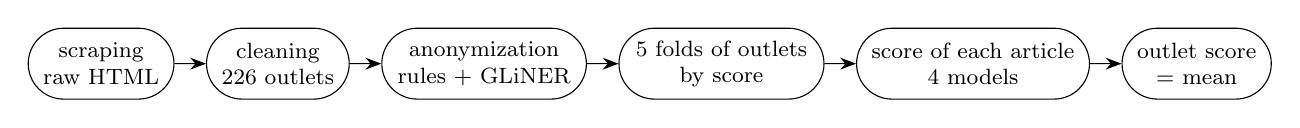
\begin{tikzpicture}[node distance=4mm, box/.style={draw, rounded rectangle, align=center, font=\footnotesize,
  minimum height=9mm, inner sep=3pt}, >={Stealth[length=2mm]}]
\node[box] (s) {scraping\\raw HTML};
\node[box, right=of s] (c) {cleaning\\226 outlets};
\node[box, right=of c] (a) {anonymization\\rules + GLiNER};
\node[box, right=of a] (f) {5 folds of outlets\\by score};
\node[box, right=of f] (m) {score of each article\\4 models};
\node[box, right=of m] (o) {outlet score\\= mean};
\foreach \x/\y in {s/c, c/a, a/f, f/m, m/o} \draw[->] (\x) -- (\y);
\end{tikzpicture}}
\caption{The pipeline.}\label{fig:pipeline}
\end{figure}

\subsection{Task and split}
Each outlet has one NewsGuard score $y \in [0, 100]$, assigned to all its articles. A model predicts a score for every
article; the score of an outlet is the mean of the predictions for its articles. Outlets are split into five folds:
outlets are sorted by score and, in consecutive blocks of five, each one goes to a different fold at random, so that
every fold has the same score distribution (Figure~\ref{fig:dataset}c). An outlet, with all its articles, is always
in a single fold, and outlets of the same owner were already reduced to one. Every model is trained on four folds and
tested on the fifth; hyper-parameters are chosen with three inner folds of the training outlets, built the same way.

\subsection{Models}
\begin{description}
  \item[TF-IDF.] Word uni- and bi-grams (at most 100,000, minimum document frequency 5, sublinear term frequency),
        fitted on the training articles, and a ridge regression; the penalty is chosen on the inner folds by the
        Spearman correlation per outlet.
  \item[Qwen3-Embedding-8B, frozen.] The embedding model \citep{zhang2025qwen3} reads every article in full with an
        instruction (\emph{``represent this news article to judge the reliability and journalistic standards of the
        outlet that published it''}); the vector of the last token, normalized, feeds a ridge regression on
        standardized features.
  \item[Mistral-Small-24B, frozen.] The base language model \citep{mistralsmall} (4-bit quantization) reads every
        article; the mean of the hidden states of layer 27 (of 40) over the article's tokens feeds a ridge
        regression, as above. \todo{say why layer 27.}
  \item[ModernBERT, fine-tuned.] ModernBERT-base \citep{warner2024modernbert} is trained end to end to regress the
        score (squared error on score/100; 5 epochs, learning rate $3\cdot10^{-5}$, effective batch 32).
\end{description}
No article is truncated: the longest one has about 3,000 tokens, below the 4,096 tokens read by every model.
All random choices are seeded and the GPU computations are deterministic; the models run on one NVIDIA V100 (32 GB).
\todo{run times?}

\subsection{Evaluation}
All measures are computed per outlet, on the 226 outlets of the five test folds: Spearman's $\rho$ and Kendall's
$\tau_b$ between predicted and true scores (the ranking of outlets), the mean absolute error (MAE, in points) and the
share of outlets predicted within 20 points of their score. The no-text baseline predicts, for every test outlet, the
mean score of the training outlets. Intervals are 95\% bootstrap intervals over outlets; differences between two
models are paired (same resampled outlets). To measure how many articles are needed, the score of each outlet is
also predicted from $k = 1, 2, 3, 5, 10, 20, 50$ random articles (20 draws per $k$, the same for every model).

% =====================================================================================================================
\section{Results}\label{sec:results}

\subsection{Main results}
Table~\ref{tab:main} reports the results with all the articles of every outlet. Without text, predicting the mean
training score gives an error of 22.6 points. All models rank the outlets far better than chance. The two frozen large
language models are the best: Mistral-Small-24B reaches a Spearman correlation of 0.735 and an error of 15.8 points, and
is significantly better than TF-IDF on every measure ($\Delta\rho = +0.060$ [0.022, 0.105]; $\Delta$MAE $= -2.0$
[$-2.8$, $-1.2$] points; $+6.6$ points in the share within 20). Qwen3-Embedding-8B significantly lowers the error
($-1.5$ [$-2.2$, $-0.7$]) and raises the share within 20 points ($+8.4$), while its rank correlation is not
significantly higher ($+0.037$ [$-0.001$, 0.077]). The fine-tuned ModernBERT is not distinguishable from TF-IDF
($\Delta\rho = -0.064$ [$-0.133$, 0.001]).

\begin{table}[t]
\centering
\caption{Predicting the NewsGuard score of unseen outlets (226 outlets, all articles). 95\% bootstrap intervals in
brackets; $^\ast$: significantly better than TF-IDF (paired bootstrap).}\label{tab:main}
\resizebox{\linewidth}{!}{%
\begin{tabular}{lcccc}
\toprule
model & Spearman $\rho$ & Kendall $\tau_b$ & MAE (points) & within 20 (\%) \\
\midrule
no text (training mean) & $-0.02$ & $-0.01$ & 22.6 [20.7, 24.6] & 50.9 [44.2, 57.5] \\
TF-IDF + ridge & 0.674 [0.60, 0.74] & 0.480 [0.42, 0.54] & 17.8 [16.1, 19.6] & 61.5 [54.9, 67.7] \\
Qwen3-Embedding-8B (frozen) + ridge & 0.711 [0.64, 0.76] & 0.514 [0.46, 0.57] & 16.3$^\ast$ [14.7, 18.0] & 69.9$^\ast$ [63.7, 75.7] \\
Mistral-Small-24B (frozen) + ridge & \textbf{0.735}$^\ast$ [0.67, 0.79] & \textbf{0.540}$^\ast$ [0.48, 0.59] & \textbf{15.8}$^\ast$ [14.3, 17.4] & 68.1$^\ast$ [62.4, 74.3] \\
ModernBERT (fine-tuned) & 0.610 [0.52, 0.68] & 0.435 [0.37, 0.50] & 17.5 [15.8, 19.3] & 63.7 [57.1, 69.9] \\
\bottomrule
\end{tabular}}
\end{table}

\subsection{How many articles are needed}
\IfFileExists{figures/curves.pdf}{%
\begin{figure}[t]
\centering
\includegraphics[width=\linewidth]{figures/curves.pdf}
\caption{Spearman correlation and MAE per outlet as a function of the number of articles read per outlet (mean of 20
random draws).}\label{fig:curves}
\end{figure}}{%
\begin{figure}[t]
\centering
\placeholder{0.9\linewidth}{4.5cm}
\caption{Spearman correlation and MAE per outlet as a function of the number of articles read per outlet.}
\label{fig:curves}
\end{figure}}
Figure~\ref{fig:curves} shows how the results grow with the number of articles read per outlet. Mistral-Small-24B is
significantly better than TF-IDF for every $k$, on both the ranking and the error: with a single article it reaches
$\rho = 0.62$ (TF-IDF: 0.39) and an error of 17.3 points (20.5), and with five articles ($\rho = 0.71$) it already ranks
the outlets better than TF-IDF reading all of them (0.67). Qwen3-Embedding-8B is significantly better than TF-IDF on
the error for every $k$ and on the ranking up to 50 articles. ModernBERT is never significantly different from TF-IDF.
All curves flatten after about ten articles.

\subsection{Robustness to the anonymization}
We ran the whole pipeline also with a simpler anonymization, made of six rules (the outlet's signature in the titles,
e-mail addresses, links, social media accounts, the outlet's own authors taken from the author field of the page, and
the outlet's name). Table~\ref{tab:anon} compares the two on the same outlets and articles. Masking every outlet and
journalist changes the language models by at most 0.011 in $\rho$ and 0.24 points of error, never significantly with
all articles; only TF-IDF loses a little ($\Delta\rho = -0.017$ [$-0.036$, $-0.001$]), consistent with TF-IDF using
names of outlets and people as features. Over all $k$ and measures, 18 of the 24 comparisons of TF-IDF are
significantly worse with the stricter anonymization, against 5 of 24 for Mistral-Small-24B and none for the other two
models. The language models therefore do not rely on explicit identifiers of the outlets.

\begin{table}[t]
\centering
\caption{Spearman $\rho$ and MAE per outlet with two anonymizations (all articles).}\label{tab:anon}
\begin{tabular}{lcccc}
\toprule
& \multicolumn{2}{c}{rules only} & \multicolumn{2}{c}{rules + GLiNER} \\
\cmidrule(lr){2-3}\cmidrule(lr){4-5}
model & $\rho$ & MAE & $\rho$ & MAE \\
\midrule
TF-IDF & 0.691 & 17.7 & 0.674 & 17.8 \\
Qwen3-Embedding-8B & 0.722 & 16.1 & 0.711 & 16.3 \\
Mistral-Small-24B & 0.735 & 15.7 & 0.735 & 15.8 \\
ModernBERT & 0.605 & 17.7 & 0.610 & 17.5 \\
\bottomrule
\end{tabular}
\end{table}

\subsection{Where the models err}
The predictions are compressed towards the centre of the scale (Mistral-Small-24B predicts outlet scores between 37
and 96). The least reliable outlets are overestimated (mean signed error for the NewsGuard level 0--39: $+31$ points
with Mistral-Small-24B, $+37$ with TF-IDF) and the most reliable ones underestimated (score 100: $-19$ and $-25$),
while the outlets in the middle of the scale (60--74) are predicted almost without bias ($-3$ and $-2$).
\todo{rank-based measures are not affected by this compression; a monotone re-calibration on the training scores would
reduce the error at the extremes.}

% =====================================================================================================================
\section{Released resources and demonstration tool}\label{sec:tool}

\paragraph{What we release.} Table~\ref{tab:release} lists the resources released with this paper
\todo{repository URLs and licences}. The NewsGuard scores and levels are licensed and are not included anywhere, not
even indirectly in the result files; the text of the articles is not redistributed either (only their URLs).

\begin{table}[t]
\centering\small
\caption{Resources released with the paper. Nothing released contains NewsGuard scores or article text.}\label{tab:release}
\begin{tabular}{p{0.24\linewidth}p{0.68\linewidth}}
\toprule
resource & content \\
\midrule
pipeline code & every step of Sections~\ref{sec:data}--\ref{sec:results}, from the raw HTML to the tables and figures \\
models & the four models of Table~\ref{tab:main}, each in its five fold versions (one per held-out fold of outlets) \\
predictions & for each of the 25,524 articles: id, URL, outlet, fold and the out-of-fold score of the four models \\
split & the 226 outlets and their fold \\
tool & \emph{Publisher Evaluation}: scores new articles with the released models (below) \\
\bottomrule
\end{tabular}
\end{table}

\paragraph{The tool.} \emph{Publisher Evaluation} runs on the user's machine (web interface and command line;
\todo{screenshot of the Evaluate page as a figure}). Given a URL or a pasted text with the domain of its outlet, it
extracts the text as in Section~\ref{sec:data} (trafilatura in precision mode) and refuses what is outside the
training data rather than extrapolating: pages that are not a single article, texts that are not in English or not
between 100 and 1,500 words. It then anonymizes the text with the procedure of Section~\ref{sec:anon} and shows it
with the placeholders highlighted, so that the user sees exactly what the models read. The user chooses which of the
available models to run; each predicts the score of the outlet from this one article, and the score of an outlet is
the mean over its stored articles, with the standard deviation and a bootstrap interval. The released predictions are
loaded from the start, so the 226 outlets of the paper can be browsed, compared across models and exported. Every
number is presented as a model prediction, not as a rating: one article is a weak signal
(Section~\ref{sec:results}).

\paragraph{Models and fidelity.} The models are shipped in formats that execute no code from the model files:
TF-IDF and the ridge heads as plain arrays, rebuilt by the tool, and ModernBERT as an ONNX graph in half precision,
as in our experiments. Against the paper's predictions, the TF-IDF scores are identical and the ridge heads differ by
less than $10^{-4}$ points on all the articles, and ModernBERT by 0.05 points on average (at most 1 point) on 1,500
checked articles; the anonymization of
the tool reproduces that of the paper exactly on a sample of 40 articles. Qwen3-Embedding-8B and Mistral-Small-24B are
downloaded once from Hugging Face and need a GPU (about 18 GB); without one, TF-IDF and ModernBERT score new articles
on a CPU (about 1 s per article and fold for ModernBERT) and the released predictions of all four models remain
available.

\paragraph{Leakage guard.} The model of fold $k$ was trained on the outlets of the other four folds. For an article
of one of the 226 outlets, the tool uses only the model of the fold that held that outlet out, so that no outlet is
scored by a model that saw it in training; for a new outlet, the score is the mean of the five fold models. An
article of the paper that is evaluated again keeps its id and is never counted twice.

\paragraph{Custom models.} Users can add their own regressors of the 0--100 score as ONNX graphs, reading either the
anonymized text or its tokens. A custom model is used only after strict checks: a valid graph with only the operators
built into ONNX and onnxruntime, exactly the declared inputs and a single score output, and a probe run on 20
synthetic anonymized articles (finite scores within the scale, not all equal, the same when scored again and when
scored in a batch). Its manifest declares which outlets it was trained on, and the same leakage guard applies (a model
that declares nothing is never used on the 226 outlets); its predictions are stored with the hash of its files and
never pooled with those of the paper's models.

% =====================================================================================================================
\section{Discussion}\label{sec:discussion}
\todo{expand.} Large language models used as frozen encoders capture more of what separates reliable from unreliable
outlets than word counts, and with far fewer articles; fine-tuning a smaller encoder on 180 training outlets does not
reach them (with so few outlets it memorizes the training outlets). The ranking of outlets is good ($\rho \approx
0.74$) but the score is predicted within 20 points only for two outlets in three: the text carries part of the
NewsGuard rating, while criteria such as the disclosure of ownership or the correction of errors are hardly visible in
the articles. The natural use is to rank unrated outlets so that human raters review the least reliable first.

\paragraph{Limitations.}
One rater (NewsGuard) at one point in time; English-language political outlets only; 226 outlets, a small number
of independent units, hence wide intervals. The anonymization removes explicit identifiers, not the writing style,
which may itself identify an outlet; the recognizer also masks some people who are not journalists (e.g.\ politicians
it takes for commentators) and misses some mentions. Predicted scores are compressed towards the centre.
\todo{expand.}

\paragraph{Ethics and data availability.}
The NewsGuard labels are licensed and are not redistributed: the released files (Table~\ref{tab:release}) contain
article ids and URLs, folds, model predictions and models, but no scores, levels or article text. The method, and the
tool built on it, are meant to support human raters, for instance by ranking unrated outlets for review, not to
replace them: the tool presents its outputs as model predictions, scores an outlet only with models that never saw
it, and runs locally, so the articles it evaluates are not sent to any third party. \todo{expand; licences of the
released models (derived from Apache-2.0 base models).}

% =====================================================================================================================
\section{Conclusion}\label{sec:conclusion}
From the anonymized text of its articles alone, the reliability of a news outlet never seen in training can be
ranked with a Spearman correlation of about 0.74 by a large language model used as a frozen encoder, significantly
better than with TF-IDF and with as few as five articles. The released models and tool let others apply the
method to new outlets and compare their own models under the same anonymization and leakage guard. \todo{polish.}

\bibliographystyle{plainnat}
\bibliography{references}

\end{document}
